\documentclass{ximera}
%% handout
%% space
%% newpage
%% numbers
%% nooutcomes

%% You can put user macros here
%% However, you cannot make new environments

\graphicspath{{./}{firstExample/}{secondExample/}}

\usepackage{tikz}
\usepackage{tkz-euclide}
\usetkzobj{all}
\pgfplotsset{compat=1.7} % prevents compile error.

\tikzstyle geometryDiagrams=[ultra thick,color=blue!50!black]
 %% we can turn off input when making a master document

\outcome{Practice with series.}
\title{An Elusive Series}
\author{Kirollos Masood}

\begin{document}
\begin{abstract}
In this activity, we tackle a historically famous series.
\end{abstract}
\maketitle

Consider this series.
\[
	\sum_{k=1}^{\infty} \frac{1}{k^2} = \frac{1}{1}+\frac{1}{4}+\frac{1}{9}+\frac{1}{16}+\ldots
\]
Does it converge? If it does converge, what's the limit? The Divergence Test fails, so that doesn't help us. If you try the Ratio Test, the result is inconclusive. However, the Integral Test comes to the rescue. Work out these details on your own and you'll see that this series must converge. Now the only issue is finding what the limit is.

\begin{exercise}	
	We will begin our journey by casting some trigonometry magic. Doesn't $\sin(x)$ have zeros at $x=0,\pi,-\pi,2\pi,-2\pi,3\pi,-3\pi,$ and so on? So what if we tried to write this as a polynomial? How about this?
	\begin{align*}
		f(x)= \left( x \right) \left( \frac{\pi-x}{\pi} \right) \left( \frac{\pi+x}{\pi} \right) \left(\frac{2\pi- x}{2\pi} \right) \left( \frac{2\pi+x}{2\pi} \right) \ldots
	\end{align*}
	Doesn't $f$ have all the same zeros as $\sin(x)$? Is this good enough as long as we have these infinitely many ``factors?'' It is true! Let's visually see what happens at different stages.
	\begin{image}
		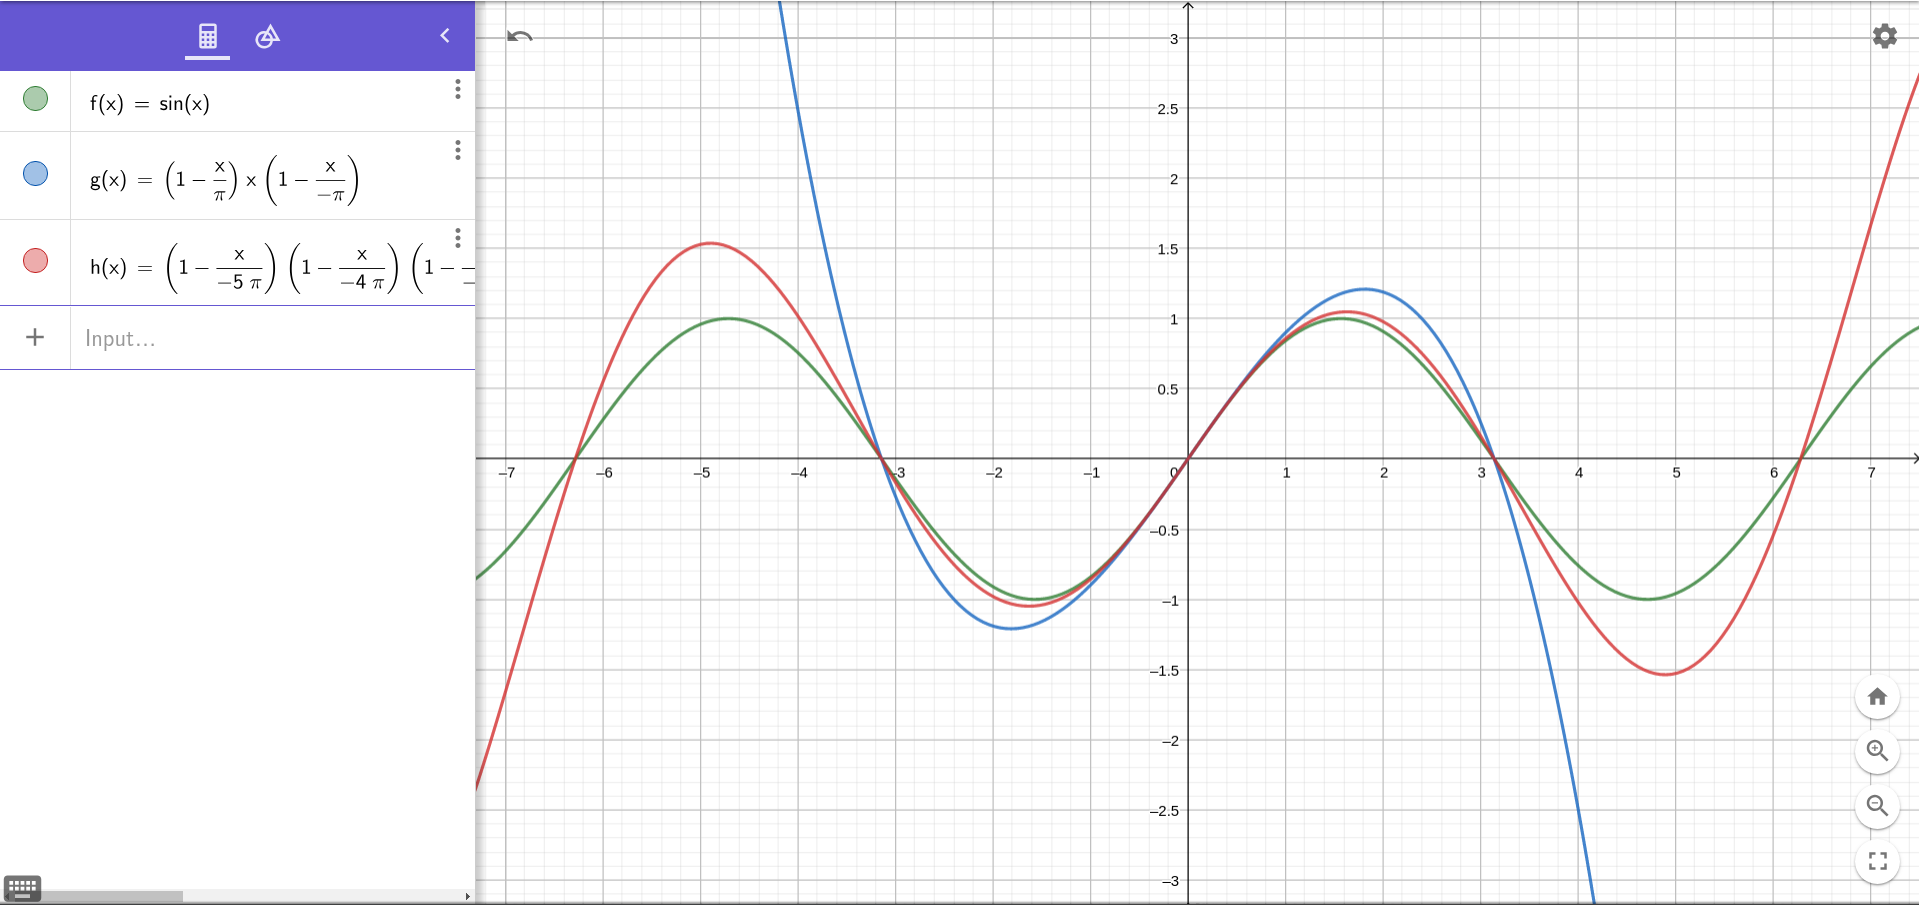
\includegraphics{sin.png}
	\end{image}
	That means we can also say the following.
	\begin{align*}
		\sin(\pi x) &= \left( \pi x \right) \left( 1-x \right) \left(1+x \right) \left(\frac{2-x}{2} \right) \left(\frac{2+x}{2} \right) \left( \frac{3-x}{3} \right) \left( \frac{3+x}{3} \right) \ldots \\
		&= \left( \pi x \right) \left( 1-x^2 \right) \left(\frac{4-x^2}{4} \right) \left(\frac{9-x^2}{9} \right) \ldots
	\end{align*}
	Alright. So we can take the natural log of both sides.
	\begin{align*}
		\ln(\sin(\pi x)) = \ln \left( \pi x \right)+\ln \left( 1-x^2  \right) +\ln \left(\frac{4-x^2}{4} \right) +\ln \left(\frac{9-x^2}{9} \right)+ \ldots
	\end{align*}
	Now take a derivative of both sides.
	\begin{align*}
		\frac{\pi \cos(\pi x)}{\sin(\pi x)} = \frac{1}{x}+\frac{-2x}{1-x^2}+\frac{-2x}{4-x^2}+\frac{-2x}{9-x^2}+\ldots \\	
	\end{align*}
	To get this to look nicer, let's move the first term on the RHS to the LHS.
	\begin{align*}
		\frac{\pi \cos(\pi x)}{\sin(\pi x)} -\frac{1}{x}= \frac{-2x}{1-x^2}+\frac{-2x}{4-x^2}+\frac{-2x}{9-x^2}+\ldots \\	
	\end{align*}
	Now divide by $-2x$.
	\begin{align*}
		\frac{-\pi \cos(\pi x)}{(2x) \sin(\pi x)} +\frac{1}{2x^2}= \frac{1}{1-x^2}+\frac{1}{4-x^2}+\frac{1}{9-x^2}+\ldots \\	
	\end{align*}
	And finally, combine the fractions on the left.
	\begin{align*}
		\frac{- (\pi x) \cos(\pi x )+\sin(\pi x)}{(2x^2)\sin(\pi x)}= \frac{1}{1-x^2}+\frac{1}{4-x^2}+\frac{1}{9-x^2}+\ldots \\	
	\end{align*}
	Hold on a moment. On the RHS, what do we get when we plug in $x=0$?
	\begin{multipleChoice}
		\choice{I don't know}
		\choice[correct]{The series we wanted!}
		\choice{0}
		\choice{Here's a wrong answer choice to provide more options.}
	\end{multipleChoice}
	But plugging in $x=0$ on the LHS leads us into dangerous territory. Thankfully, we are armed with L'Hospital's Rule. (You might have to swing the sword of L'Hospital repeatedly.) So then, you tell me:
	\begin{align*}
		\sum_{k=1}^{\infty} \frac{1}{k^2} = \answer[given]{\frac{\pi^2}{6}}	
	\end{align*}
\end{exercise}


\end{document}
